\documentclass[12pt,a4]{article}




\usepackage{graphicx,amsmath,amssymb,amsthm, boxedminipage,xcolor,amscd,amsbsy,latexsym,url,bm}

%\usepackage[lined,boxed]{algorithm2e}

\usepackage{algorithm}
\usepackage{algpseudocode}


\newtheorem{theorem}{Theorem}[section]
\newtheorem{proposition}[theorem]{Proposition}
\newtheorem{lemma}[theorem]{Lemma}
\newtheorem{corollary}[theorem]{Corollary}
\newtheorem{definition}[theorem]{Definition}

\newtheorem*{theorem*}{Theorem}
\newtheorem*{lemma*}{Lemma}
\newtheorem*{solution}{Solution}
\newtheorem*{proposition*}{Proposition}


\newtheorem{exercise}[theorem]{Exercise}
\newtheorem{exerciseD}[theorem]{*Exercise}
\newtheorem{exerciseDD}[theorem]{**Exercise}

\let\oldexercise\exercise
\renewcommand{\exercise}{\oldexercise\normalfont}

\let\oldexerciseD\exerciseD
\renewcommand{\exerciseD}{\oldexerciseD\normalfont}

%\let\oldexerciseD\exerciseD
%\renewcommand{\exerciseD}{\oldexerciseD\normalfont}

%\let\oldexerciseDD\exerciseDD
%\renewcommand{\exerciseDD}{\oldexerciseDD\normalfont}

\newcommand{\E}{\mathbb{E}}
%\newcommand{\nth}[1]{#1^{\textsuperscript{th}}}
\newcommand{\scalar}[2]{\ensuremath{\langle #1, #2\rangle}}
\newcommand{\floor}[1]{\left\lfloor #1 \right\rfloor}
\newcommand{\ceil}[1]{\left\lceil #1 \right\rceil}
\newcommand{\norm}[1]{\|#1\|}
\newcommand{\pfrac}[2]{\left(\frac{#1}{#2}\right)}
\newcommand{\nth}[1]{#1^{\textsuperscript{th}}}
\newcommand{\core}{\textnormal{core}}



\newif\ifsolution

\solutionfalse

\newcommand{\answer}[1]{
\ifsolution
{\color{blue} #1}
\else
\fi
}



\newcommand{\poly}{\textnormal{poly}}
\newcommand{\quasipol}{\textnormal{quasipol}}
\newcommand{\ssubexp}{\textnormal{stronglySubExp}}
\newcommand{\wsubexp}{\textnormal{weaklySubExp}}
\newcommand{\simplyexp}{\textnormal{E}}
\newcommand{\expo}{\textnormal{Exp}}



\newcommand{\N}{\mathbb{N}}
\newcommand{\nn}{\mathbb{N}_0^n}
\newcommand{\R}{\mathbb{R}}
\newcommand{\Z}{\mathbb{Z}}


\definecolor{darkgreen}{rgb}{0,0.6,0}

\date{}

\title{
\hbox{  Mathematical Foundations of Computer Science}
  \vspace{3mm}
{\normalsize CS 499,	Shanghai Jiaotong University,  Dominik Scheder\\
%\vspace{3mm}
Spring 2019}
}


\begin{document}

\maketitle

%\begin{quotation}
%  You are welcome to discuss the exercises in the discussion
%  forum. Please take them serious. Doing the exercises is as important
%  than watching the videos.
%
%  I intentionally included very challenging exercises and marked them
%  with one or two ``$*$''. No star means you should be able to solve
%  the exercises without big problems once you have understood
%  the material from the video lecture. One star means it requires 
%  significant additional thinking. Two stars means it is not 
%  unlikely that you will fail to solve them, even once you have understood
%  the material and thought a lot about the exercise. Don't feel bad
%  if you fail. Failure is part of learning.
%
%  This is the first time this course is online. Thus there might be mistakes
%  (typos or more serious conceptual mistakes) in the exercises. I will be 
%  grateful if you point them out to me!
%\end{quotation}



\setcounter{section}{9}

\section{Network Flow}



\begin{itemize}
 \item Homework assignment published on Thursday 2019-05-16
 \item Submit questions and first solution by Wednesday, 2019-05-22, 12:00
 \item Submit final solution by Wednesday, 2019-05-29.
\end{itemize}


\begin{exercise}[From the video lecture]
   Recall the definition of the value of a flow: ${\rm val}(f) = \sum_{v \in V} f(s,v)$.
   Let $S \subseteq V$ be a set of vertices that contains $s$ but not $t$. Show that
   \begin{align*}
         {\rm val}(f) = \sum_{u \in S, v \in V \setminus S} f(u,v) \ .
   \end{align*}
   That is, the total amount of flow leaving $s$ equals the total amount of flow 
   going from $S$ to $V \setminus S$.
   \textbf{Remark.} It sounds obvious. However, find a formal proof that works with the 
   axiomatic definition of flows. 
\end{exercise}

\begin{proof}
	$$
		{\rm val}(f) = \sum_{u \in S, v \in V \setminus S} f(u,v) = \sum_{e \text{ out of } S} f(e) - \sum_{e \text{ in to } S} f(e)
	$$
	$
		\sum\limits_{e \text{ out of } v} f(e) = \sum\limits_{e \text{ in to } v} f(e)
	$, if $v \neq s, t$. \\
	Thus,
	\begin{align*}
		{\rm val}(f) &= \sum_{e \text{ out of } s} f(e) - \sum_{e \text{ in to } s} f(e) \\
		&= \sum\limits_{v \in S}(\sum\limits_{e \text{ out of } v}f(e) - \sum\limits_{e \text{ in to } v}f(e)) \\
		&= \sum_{e \text{ out of } S} f(e) - \sum_{e \text{ in to } S} f(e) \\
		&= \sum_{u \in S, v \in V \setminus S} f(u,v)
	\end{align*}
	\end{proof}

\begin{exercise}
Let $G = (V,E,c)$ be a flow network.
  Prove that flow is ``transitive'' in the following sense: 
  If there is a flow from $s$ to $r$ of value $k$,
  and a flow from $r$ to $t$ of value $k$, then
  there is a flow from $s$ to $t$ of value $k$.
  \textbf{Hint.} The solution is extremely short. If you are trying
  something that needs more than 3 lines to write, you are on the wrong
  track.
\end{exercise}

\begin{proof}
	A flow from $s$ to $r$ of value $k$: $k = \sum\limits_{e \text{ in to } r}f(e)$ \\
	A flow from $r$ to $t$ of value $k$: $k = \sum\limits_{e \text{ out of } r}f(e)$ \\
	Then there must be a flow from $s$ to $t$ of value $k$.
\end{proof}

\subsection{An Algorithm for Maximum Flow}

Recall the algorithm for Maximum Flow presented in the video. It is usually called
the Ford-Fulkerson method.

\begin{algorithm}[h]
\caption{Ford-Fulkerson Method}\label{algorithm-encoding}
\begin{algorithmic}[1]
\Procedure{FF}{$G=(V, E), s, t, c$} 
  \State Initialize $f$ to be the all-$0$-flow.
   \While{there is a path $p$ form $s$ to $t$ in the residual network $G_{f}$}
    \State $c_{\rm min} := \min \{ c_f(e) \ | \ e \in p \}$ 
    \State let $f_p$ be the flow in $G_f$ that routes $c_{\rm min}$ flow along $p$
    \State $f:= f + f_p$
   \EndWhile
   \State \texttt{//} now $f$ is a maximum flow
  \State $S := \{v \in V \ | \ G_f \textnormal{ contains a path from } s \textnormal{ to } v \}$
  \State \texttt{//} $S$ is a minimum cut
  \State \Return $(f,S)$
\EndProcedure
\end{algorithmic}
\end{algorithm}

We proved in the lecture that $f$ is a maximum flow and $S$ is a minimum cut,
by showing that upon termination of the while-loop, ${\rm val}(f) = {\rm cap}(S)$.
The problem is that the while-loop might not terminate. In fact, there is an example
with capacities in $\mathbb{R}$ for which the while loop does not terminate, and the 
value of $f$ does not even converge to the value of a maximum flow. As indicated
in the video, a little twist fixes this:
\begin{quotation}
  \textbf{Edmonds-Karp Algorithm:} Execute the above 
  Ford-Fulkerson Method, but in every iteration choose $p$ to be a 
  shortest $s$-$t$-path in $G_f$. Here, ``shortest'' means minimum number of edges.
\end{quotation}
In a series of exercises, you will now show that this algorithm always terminates
after at most $n \cdot m$ iterations of the while loop (here $n = |V|$ and $m = |E|$).

\begin{definition}
   Let $(G,s,t,c)$ be a flow network and $k \in \mathbb{N}_0$.
   A {\em $k$-layering} is a partition of $V = V_0 \cup \dots \cup V_k$ such that
   (1) $s \in V_0$, (2) $t \in V_k$, (3)
   for every edge $(u,v) \in E$ the following holds: suppose $u \in V_i$ and $v \in V_j$.
   Then $j \leq i+1$. 
   In words, point (3) states that every edge moves at most one level forward.
\end{definition}

The figure below illustrates this concept: for one network we show two possible layerings
and something that looks like a layering but is not:
\begin{center}
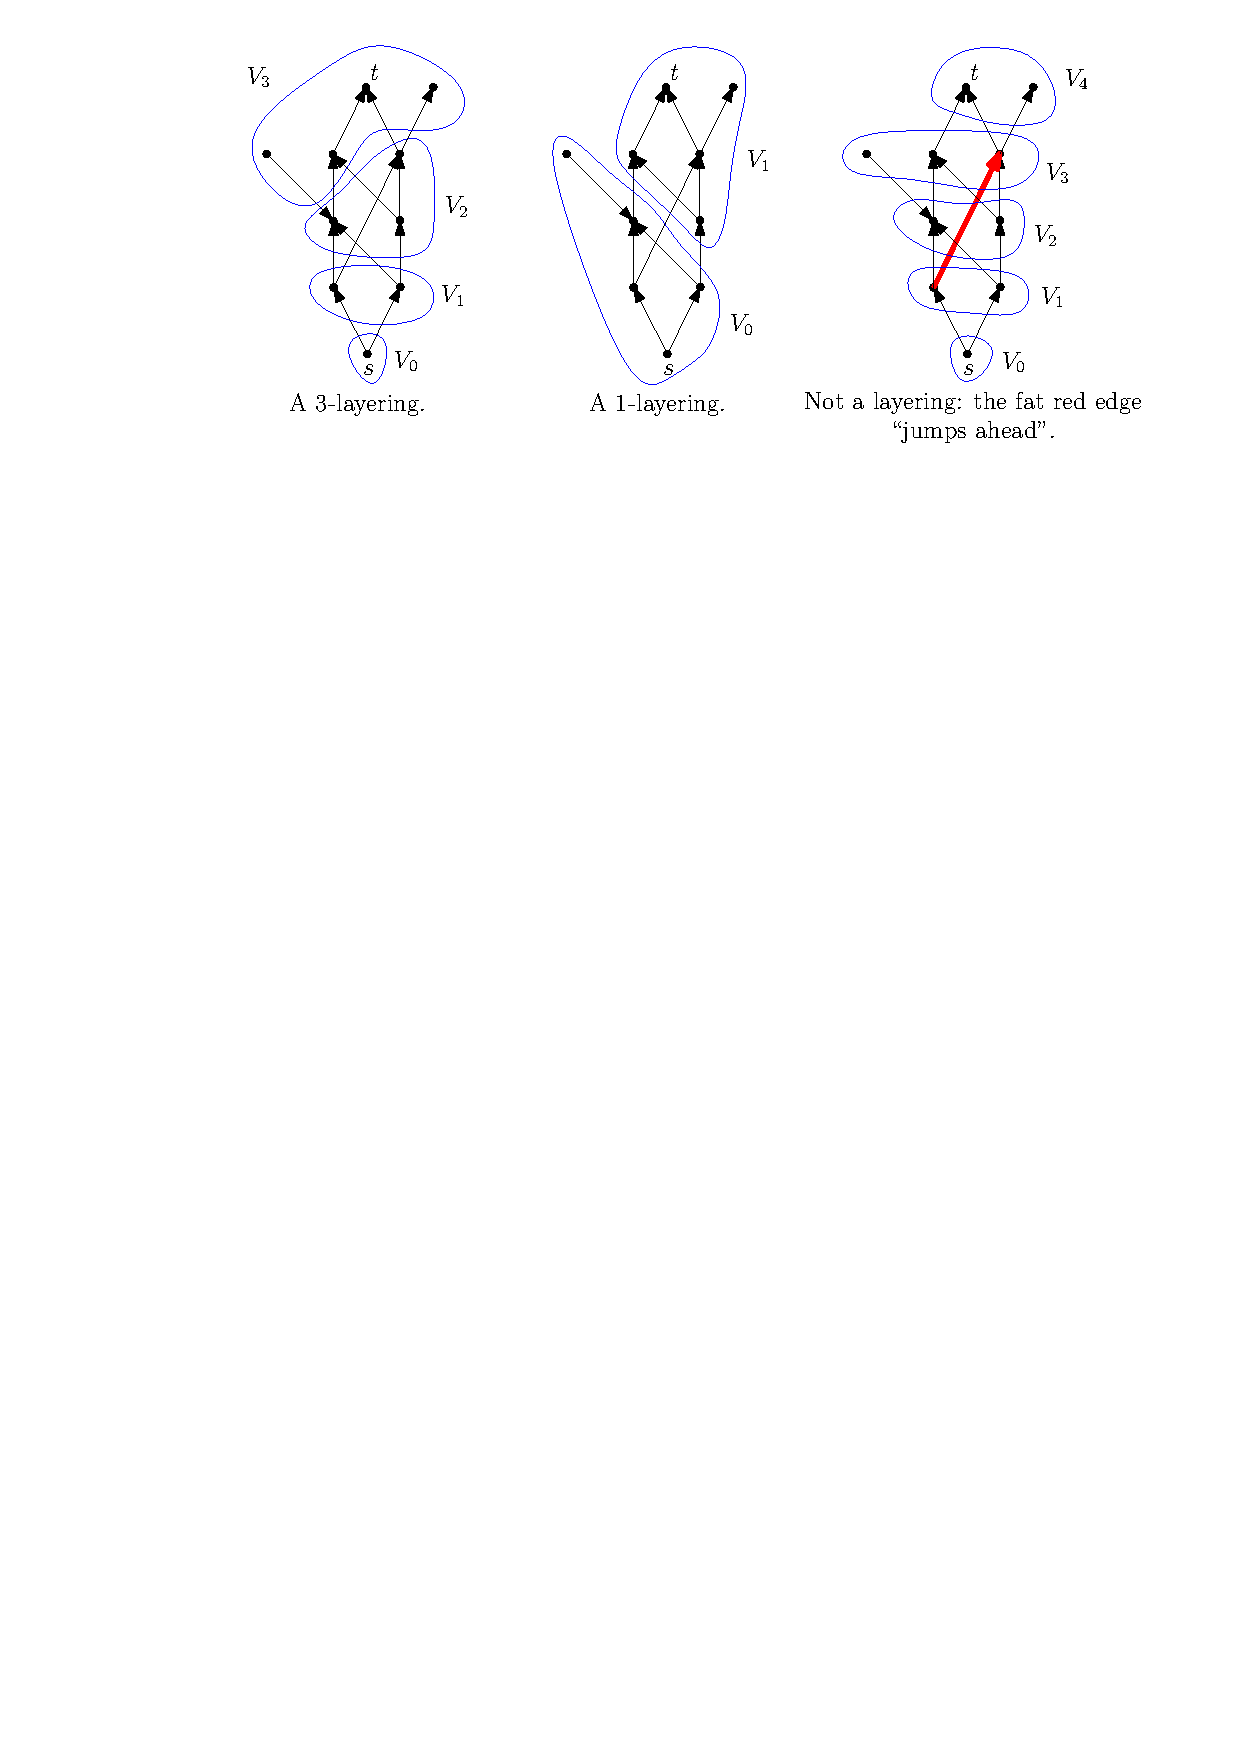
\includegraphics[width=\textwidth]{figures/layering.pdf}
\end{center}

\begin{exercise}
   Suppose the network $(G,s,t,c)$ has a $k$-layering. Show that ${\rm dist}(s,t) \geq k$.
   That is, every $s$-$t$-path in $G$ has at least $k$ edges.
\end{exercise}

\textbf{Proof.} \quad \textbf{Claim:} With $i$ edges, a path starting from $s$ can reach at farthest a vertex in $V_i$ in $k-$layering ($1\leq i\leq k$).

\textbf{Proof of claim:} Suppose the claim does not hold. That is, there is some path starting from $s$ with $i$ edges that can reach a vertex in $V_j$, $i<j\leq k$. And we know that $S$ is in $V_0$. Then there must exist some edge $(u,v)$, $u\in V_m,v\in V_n$ such that $n-m>1$ in the path, which violates the definition of layering. \qed

Let $i\leq k-1$ and we get that with less than $k$ edges, a path starting from $s$ can reach at farthest a vertex in $V_{k-1}$, but can never reach a vertex in $V_k$. To reach $t\in V_k$, the path must include at least $k$ edges. \qed 

\begin{exercise}
   Conversely, suppose ${\rm dist}(s,t) = k$. Show that $(G,s,t,c)$ has a $k$-layering.
\end{exercise}

\textbf{Proof.} \quad\textbf{Claim:} Algorithm~\ref{alg:k-layering} outputs a $k-$layering for dist($s,t$)=$k$.\newline

   \begin{algorithm}[H]
      \caption{Algorithm to output a $k-$layering for dist($s,t$)=$k$}\label{alg:k-layering}
      \begin{algorithmic}[1]
      \Procedure{$k$-layering}{$G=(V, E), s, t, c$,dist($s,t$)=$k$}
      \State grab a shortest path $p=(V',E')$ from $s$ to $t$
      \State sort $V'$ according to the sequence of visiting on the path
      \ForAll{vertex $v_i\in V'$} 
        \State $V_i\leftarrow\{v_i\}$
      \EndFor
      \For{$i\leftarrow k$ to $1$} 
         \ForAll{edge $(u,v)\notin E'$ with $v\in V_i$} 
           \State add $u$ to $V_{i-1}$
         \EndFor
      \EndFor
     \State \Return $V_0,V_1,\cdots,V_k$
     \EndProcedure
\end{algorithmic}
   \end{algorithm}


\textbf{Proof of claim:} Clearly $s\in V_0$ and $t\in V_k$ according to this algorithm. We just need to prove that for every edge $(u,v)\in E$, $u\in V_i,$ $v\in V_j$, $j\leq i+1$.

First for every edge $(u,v)\in E'$ in $p$, according to the algorithm, we have $j=i+1$ exactly, which satisfies the requirement. Then for edges not in $p$, suppose some edge has that $j>i+1$. Then we can delete at least two edges in the shortest path: one from $V_i$ to $V_{i+1}$ and another from $V_{i+1}$ to $V_j$, replace them with the very special edge, and thus we get a shorter path than the shortest path $p$. Therefore all edges in $E$ satisfy $j\leq i+1$.\qed 

Since Algorithm~\ref{alg:k-layering} returns a $k$-layering for the network $(G,s,t,c)$, $(G,s,t,c)$ has a $k$-layering.\qed
\vspace{10pt}

Let $(G,s,t,c)$ be a flow network and $V_0,\dots,V_k$ a $k$-layering. We call this 
layering {\em optimal} if ${\rm dist}_G(s,t) = k$. Here, ${\rm dist}_G(u,v)$ 
is the shortest-path distance from $s$ to $t$ (measured by number of edges).
If there is no path from $s$ to $t$, we set ${\rm dist}_G(s,t) = \infty$. In this case, 
no layering is optimal.
For example, the $3$-layering
in the above figure is optimal, but the $1$-layering in the middle of the above figure
is not.
Let us explore how layerings and the Ford-Fulkerson Method interact.

\begin{exercise}
   Let $(G,s,t,c)$ be a flow network and $V_0, V_1, \dots, V_k$ be an optimal layering
   (that is, $k = {\rm dist}_G(s,t)$.
   Let $p$ be a path from $s$ to $t$ of length $k$. 
   Suppose we route some flow $f$ along $p$ (of some
   value $c_{\rm min} > 0$) and let $(G_f,s,t,c_f)$ be the residual network. Show that
   $V_0, V_1,\dots, V_k$ is a layering of $(G_f,s,t,c_f)$, too. Obviously, condition (1) and (2) in
   the definition of $k$-layerings still hold, so you only have to check  condition (3).
\end{exercise}

%----------------------------------BEGIN----------------------------------
\textbf{Solution.} For the residual network, we assume it violates condition (3), i.e., there exist an edge moves at least 2 levels forward. However, this edge doesn't exist in the original network. By the definition of residual network, we add an edge only if there exist an edge between the corresponding two vertices in the original graph. That is a contradiction. Then we claim there is no edge moves at more than 1 level forward in the residual network.
%-----------------------------------END-----------------------------------

\begin{exercise}
   Show that every network $(G,s,t,c)$ has an optimal layering, provided there is a path
   from $s$ to $t$.
\end{exercise}

%----------------------------------BEGIN----------------------------------
\textbf{Solution.}
Consider vertices in $G$, there are three types of vertices. For the first type $v \in V$, there exist both a path $s\rightarrow v$ and a path $v\rightarrow t$. Let the set of such vertices be $V_{reduce}$. \par 
For the second type $v \in V$, there exist a path $s\rightarrow v$, but no path $v \nrightarrow t$. Let the set of such vertices be $V_{out}$.\par 
For the second type $v \in V$, there exist a path $v\rightarrow t$, but no path $s \nrightarrow v$. Let the set of such vertices be $V_{in}$.
$$V = V_{reduce} \cup V_{out} \cup V_{in}$$\par 
 For $v\in V_{reduce}$, by definition, it's reachable for $s$. Let $c = dist_{G}(s,v)$ (the shortest distance from $s$ to $v$). Then we assign $v$ to $c^{th}$ level $V_c$. In this way, no edge moves at more than 1 level forward. Otherwise, if we let $(v_1,v_2)\in E$, $c = dist_{G}(s,v_1)$, $c+2 = dist_{G}(s,v_2)$, it's a contradiction because there exist a path $s\rightarrow v_1 \rightarrow v_2$ whose length is $c+1$.\par 
 For each $v'\in V_{in}$, there exist at least one vertex in $V_{reduce}$ that $v'$ can first reach to. Among those vertices we choose the vertex in the highest layer. Then we assign $v'$ to that layer.\par 
  For each $v'\in V_{out}$, there exist at least one vertex in $V_{reduce}$ that $v'$ can first connect to $v'$. Among those vertices we choose the vertex in the lowest layer. Then we assign $v'$ to that layer.\par 
 Therefore, every network $(G,s,t,c)$ has an optimal layering, provided there is a path from $s$ to $t$.
 %-----------------------------------END-----------------------------------

\begin{exercise}
   Imagine we are in some iteration of the while-loop of the Edmonds-Karp algorithm.
   Let $V_0, \dots, V_k$ be an optimal layering of $(G,s,t,c)$. Show that after at most $m$
   iterations of the while-loop, $V_0,\dots,V_k$ ceases
   to be an optimal layering. \textbf{Remark.} Note that it is the {\em network} that changes from
   iteration to iteration of the while-loop, not the partition $V_0,\dots,V_k$. We consider
   the partition $V_0,\dots,V_k$ to be fixed in this exercise.
\end{exercise}

\begin{proof}
  From the previous definition of the layering, we know that any flow $f$ cannot pass the partition forwarding. This means that flow cannot go from $V_i$ to $V_j$ $(j>i+1)$ directly. For $m=|E|$, there is at most $m$ edges from $V_i$ to $V_{i+1}$. Therefore, after at most $m$ iterations, if more flows wat to pass the partition, they need to go back from $V_{i+1}$ to $V_j$ $(j \leq i+1)$. This makes $dist(s,t) >k$ and $V_0,\cdots,V_k$ no long an optimal layering, which leads to a contradiction.

\end{proof}
\begin{exercise}
Show that the Edmonds-Karp algorithm terminates after $n \cdot m$ iterations of the
while-loop. \textbf{Hint.} Initially, compute an optimal $k$-layering (which?). Then keep
this layering as long as its optimal. Once it ceases to be optimal, compute a new optimal
layering. Note that the Edmonds-Karp algorithm does not actually need to compute any
layering. It's us who compute it to show that $n \cdot m$ bound on the number of iterations.
\end{exercise}

\begin{proof}
  Since Edmonds-Karp Algorithm is a special case of Ford-Fulkerson Algorithm, from Exercise 8 we know that after at most $m$ iterations of the while-loop, $V_0,\cdots,V_k$ will cease to be an optimal layering. That is, $dist(s,t)$ is no longer $k$.\par
  As shown above, Edmonds-Karp Algorithm always choose $p$ to be the shortest path from $s$ to $t$. Then $dist(s,t)=k'$ is now at least $k+1$. We have $1 \leq k \leq n$, we can find a new optimal layering at most $n$ times.\par
  Hence the Edmonds-Karp Algorithm terminates after $n \cdot m$ iterations of while-loop.
\end{proof}

\begin{exercise}
   Show that every network has a maximum flow $f$. 
   That is, a flow $f$ such that ${\rm val}(f) \geq {\rm val}(f')$ for every flow $f'$.
   \textbf{Remark.} This sounds obvious but it is not. In fact, there might be an infinite
   sequence of flows $f_1, f_2, f_3, \dots$ of increasing value that does not reach any maximum.
    Use the previous exercises!
\end{exercise}

\begin{proof}
	Suppose that some network don't have a maximum. Then, there must exist one augmenting path from $s$ to $t$. Then we can use Edmonds-Karp algorithm to deal with this situation. From previous exercise, we have proved that this algorithm terminates after limited number of iterations. When it terminates, we successfully get the maximum flow $f$.
\end{proof}



\end{document}
